\chapter{Systematic Literature Review}
\label{chapter:SLR}

In this chapter, to answer the question ``What is the current state of language workbenches supporting projectional editing?'' we embarked on a systematic literature review (SLR).
In section \ref{section:slr_method}, we describe the method of this SLR.
Section \ref{section:slr_result} examines the outcome of our research.
Finally, in section \ref{section:slr_discussion}, we discuss the threats to the validity of our approach. 

\section{Method}
\label{section:slr_method}

To answer the first Research Question, ``what is the current state of Projectional Editing?'' we conducted a systematic literature review.
Hereafter, we describe the method we undertook. 
We followed Kitchenham's\cite{kitchenham2015evidence} advice on systematic literature review protocol validation to carry out this review.

\subsection{Motivation}
The motivation that preceded this research was a requirement to understand if projectional editing was an idea that was worth investigating.
Our background research showed an interest in the precursors to projectional editing in the late '70s through to the mid-'80s.
Outside of academia, interest arose in the mid-'90s following Charles Simonyi's treaties on Intentional programming.
However, Simonyi's call to arms did not lead to a swell in academic research as his company's product, Intentional Domain Workbench, was a closed commercial product.
Conversely, after JetBrain's opensource Meta Programming System (MPS) release, in the late 2000s, there was a flurry of papers on the subject.

Is there a need for a study of this topic? 
We believe, at least in the microcosm of this master's project, it is helpful to know whether we are researching in a dying or vibrant area.

There does not seem to be any recent SLRs specifically about projectional editing.
This study is not extending any previously conducted SLR.
Although there exist literature surveys and mapping studies in some adjacent fields, we found no SLRs.
Thus, we believe it may be helpful for those in the language engineering research community to bring together all current research about projectional editing in one place.

\subsection{Research Question}
We try to answer the question "What is the current state of Projectional Editing?" with an SLR. 
We have broken this question into three sub-questions.

\begin{itemize}
    \setlength\itemsep{0em}
    \item \textbf{Sub Question 1} ``Is there any current research in the area of projectional editing?''
    \item \textbf{Sub Question 2} ``Which tools are currently being used for research?''
    \item \textbf{Sub Question 3} ``What is the sentiment in papers currently discussing projectional editing?''
\end{itemize}


\subsection{Search Strategy}

The search process is automated as SLRs require a high level of completeness, which one cannot effectively achieve manually.
Our first major decision was whether to engage in creating a quasi-gold standard as advised by Zhang\cite{Zhang_2011}.
Zhang noted that the ad-hoc nature of search strategies in SLRs has limitations.
We executed a preliminary ad-hoc search to try and ascertain the extent of the research space.
After satisfying that the research space was small enough, we decided against using the Quasi-Gold standard, which was overkill for our requirements.

The search terms we landed on were as follows:
\begin{lstlisting}[frame=none]
     ``PROJECTIONAL EDITING'' 
      OR 
     ``PROJECTIONAL EDITOR'' 
\end{lstlisting}

We adjusted these search terms to fit the query syntax of the various search engines.

As most research search engines offer date ranges, we also used the date range to eliminate unnecessary papers at the automated search stage to save the effort of excluding them later.
In our research question, we are specifically looking at the current state of projectional editing.
A restriction of many research search engines is that they define date ranges in whole years.
When designing our search strategy, it was near the beginning of 2021.
We concluded that only including papers from 2021 would be too small a search space. 
Therefore, we set our date range to be from the beginning of 2020 to the present.
For the sake of reproducibility, we advise the removal of any papers after 31st July 2021.

\begin{table}
    \begin{center}         
        \begin{tabular}{|l||l|}
            \hline
            ACM digital library       & Google Scholar       \\
            \hline
            BASE                      & CORE                 \\
            \hline  
            IEEE Xplore               & ISI Web of Science   \\
            \hline  
            Microsoft Academic        & Science.gov          \\
            \hline  
            Wiley InterScience        & SCOPUS               \\
            \hline  
            Semantic Scholar          & SpringerLink         \\
            \hline  
        \end{tabular}
    \end{center}
    \caption{Search engines used}
    \label{table:searchEngines}
\end{table}

We show the search engines we used in table \ref{table:searchEngines}.

Once we have filtered the automated search through the criteria of the selection stage, we will use that as our starting set for snowballing.
We will do all our filtering before we do any quality assessments, as we feel that excluding papers from snowballing based on the quality of the primary study would artificially limit the network of potential papers.
Our snowballing procedure shall follow the advice of Wohin\cite{Wohlin_2014}.
Snowballing is a technique for finding related papers using the reference lists in our starting set and applying the same selection criteria.

Where possible, we will get the forward snowballing papers from the ``cited by'' functionality of Google Scholar.
Because of the range of the search being ``to present'', all papers that cite the target paper will fall within our criteria.
For backward snowballing, we will manually filter the bibliography section of the selected papers, selecting any paper published in 2020 or 2021

After gathering all the papers from the forward and backwards snowballing, we will apply the selection criteria again.
The snowballing process will recursively iterate until there are no new papers.
The papers accepted in each iteration will form the basis for the following stage - the quality assessment of the primary studies.

After the final iteration, as a final step, the selected papers will have a deeper scan. 
This deep scan ensures that the papers selected in our initial scan all meet our inclusion criteria before moving on to the quality assessment.

\subsection{Study Selection}

The inclusion criteria are:
\begin{itemize}
    \setlength\itemsep{0em}
    \item Studies are about or mention projectional editing or one of its synonyms.
    \item The study published date is in the period 2020-2021.
\end{itemize}

The exclusion criteria are:
\begin{itemize}
    \setlength\itemsep{0em}
    \item Books and grey literature.
    \item Not in English.
    \item Full text unavailable.
    \item Papers with severe issues with grammar or vocabulary.
    \item A duplicated paper.
    \item The primary study is in a previously selected paper.
\end{itemize}

If multiple papers look at the same study with different approaches, we aggregate the data during the synthesis stage.

As a lone researcher, we must be aware of bias in positively including relevant papers and excluding irrelevant papers.
We will follow Kitchenham's suggestions to overcome such bias:
\begin{itemize}
    \setlength\itemsep{0em}
    \item Test-retest 
    \begin{itemize}
        \setlength\itemsep{0em}
        \item We will assess the papers once (on title abstract and keywords) against the inclusion and exclusion criteria.
        \item Save all the suggested results.
        \item Assess the papers again three days later in a different order to the first.  
    \end{itemize}
    \item If there are disagreements, we will use Cohen's\cite{Cohen_1960} Kappa agreement statistic to see if the process needs to be refined.
\end{itemize} 

If our searches appear too large for a lone researcher, we will turn to text mining.
We will be cautious about using this.
O'Mara-Eves et al.'s\cite{OMara-Eves_2015} systematic review of text mining in systematic reviews recommends using this for prioritisation but finds that for exclusion screening, although promising, it is not yet proven.

An SLR is interested in studies rather than papers.
There is a many-to-many relation between papers and studies.
We will review the selected papers to note when this has happened in our results to make sure studies do not get over or undercounted.

\subsection{Quality of Primary Studies}
To discover explanatory reasons for why there may be differences in study results and to weigh how valuable specific studies are, we will assess the quality of the selected studies.

To avoid a ``Results Section bias'', we will be operating a results-blind quality assessment.
We base our study quality on the methods section of the papers only.
However, this bias is still a threat because the abstract, which we will read, summarises the results.
The study quality will not be measured until after the selection process is complete, though it will, in part, occur before the selection re-test process.

To conduct the quality assessments, we will use checklists from the Center for Evidence-Based Management, found in Appendix \ref{appendix:QualityAssesmentChecklist}.
These checklists address general scientific research.

In software engineering, many studies fall under what Gregor\cite{gregor2006nature}, in ``A Taxonomy of Theory Types in Information Systems Research'', calls ``Type V: Theory for Design and Action''.
These types of studies are also known as Action Design Research (ADR).

The checklists do not address this type of research well.
On investigating how other SLRs conduct a quality assessment of ADR studies, we did not find a solution.
Therefore, we will continue with the checklists shown in the appendix, using the checklists meant for Case Studies for the ADR research papers.
We will take this into account before dismissing results of this type based on their quality score.

As a lone researcher will carry out this study, there is no need to have a process for disagreements between researchers.

We use the quality assessment checklist to weed out the biases of selection, performance, detection, exclusion, and other threats to the validity of the studies under test.


\subsection{Data Extraction}
\label{section:dataExtraction}
No data extraction will be necessary for the first sub-question,  ``Is there current research in the area of projectional editing?''.
The existence of papers with verified primary studies either into projectional editing theory or its practical use will be enough to answer the question.

For the question of ``What tools are currently being used for research?'' we shall note each tool discussed mentioned explicitly in the study.

\noindent\begin{minipage}{\textwidth}
    \begin{lstlisting}[language=Python, numbers=left, caption=Text Analytics code, captionpos=b, label=listing:text_analytics, breaklines=true]

    from azure.core.credentials import AzureKeyCredential
    from azure.ai.textanalytics import TextAnalyticsClient
    
    endpoint = "REPLACE_WITH_CORRECT_ENDPOINT"
    key = "REPLACE_WITH_CORRECT_KEY"
    
    text_analytics_client = TextAnalyticsClient(endpoint=endpoint, credential=AzureKeyCredential(key))
    
    inputfiles = [[ARRAY_OF_FILES_TO_BE_ANALYSED]]
    
    with open('/content/sample_data/sentiment/output_all.txt','a') as outf:
    for sections in inputfiles:
        for section in sections:
        print("Section: {}".format(section),file=outf)
        f = open('/content/sample_data/sentiment/'+section)
        content = f.readlines()
        # for brevity an optimization to deal with 10 document limit is removed
        if len(content) != 0:
            result = text_analytics_client.analyze_sentiment(content, show_opinion_mining=True)
            docs = [doc for doc in result if not doc.is_error]
            for idx, doc in enumerate(docs):
            print("sentiment: {}".format(doc.sentiment),file=outf)
            print("Document text: {}".format(content[idx]),file=outf)
    \end{lstlisting}
\end{minipage}

Finally, for the sentiment, we shall pass each paragraph of the introduction, the discussion, the conclusion, and any other sections that mention projectional editing or tools through a sentiment analyser, noting its sentiment score.
The sentiment analysis tool we shall use is Microsoft Azure Cognitive Services Text Analytics.
We show the code to carry out this task in listing \ref{listing:text_analytics}.

\begin{table}
	\centering
	\begin{tabular}{|c | l | l | c |} 
		\hline
		\#& Data Type           & Description                                          & RQ     \\ \hline
		\hline
        1 & Study ID            & Unique identifier for the study                      &        \\ \hline
        2 & Title of Study      & The paper name                                       &        \\ \hline
        3 & Year of Publication & Will be either 2020 or 2021                          &        \\ \hline
        4 & Author(s) Names     &                                                      &        \\ \hline
        5 & Source of Study     & Name Of Online Database/ Digital Library             &        \\ \hline
        6 & Type of Study       & Experiment/Case Study/Survey/ADR            &        \\ \hline
        7 & Name of Venue       & Journal/Conference in which study has been published &        \\ \hline
        8 & Tools in Study      & A list of the tools used                             & RQ 1.2 \\ \hline
        9 & Sentiment           & The sentiment scores from appropriate paragraphs     & RQ 1.3 \\ \hline		
	\end{tabular}	
	\caption{Data extraction form}
    \label{table:Data_Extraction_Form}
\end{table}

We will gather this data in tables with the categories shown in table \ref{table:Data_Extraction_Form}.

\subsection{Data Aggregation and Synthesis}
Kitchenham\cite{kitchenham2015evidence} explained that primary studies would tend to be too heterogeneous for any statistical analysis in software engineering. 
Synthesising outcomes from multiple methods will be complex.
Thus, our synthesis will take a narrative approach.

Narrative synthesis tells a story of the who, how, and why of the success or otherwise of the research.
For ADR research, the focus will be on what will help or hinder the adoption of the implementations.
It will also examine how reliable the results are and the relationships between the studies.



\section{Results}
\label{section:slr_result}

We carried out a systematic literature review (SLR).
We summarise the results of our SLR as ``undetermined''.
We make this statement because the review design was not wholly appropriate for the problem domain.

We could not find a quality assessment checklist that adequately dealt with design science research (DSR) studies.
This inadequacy proved problematic, as most of the primary studies were DSR studies.
Therefore, what follows should be considered the results of a quasi-SLR, with the quality assessment stage ignored.

\subsection{Papers Selected}
We logged the details of what we describe in this section in appendix \ref{Appendix:SLRLog}.

Figure \ref{fig:search_results}, on the following page, shows the results of the five iterations that the search went through.
Out of 173 results, we had 50 papers that provisionally seemed to pass our inclusion and exclusion criteria from our initial search.
From the initial 50, we added 18 papers from a possible 109 in our first iteration of forward and backwards snowballing.
The next snowballing iteration returned three papers that matched our criteria.
The third round of snowballing had no papers matching our criteria and thus terminated this stage of selection.

\begin{figure}
    \centering
    \fbox{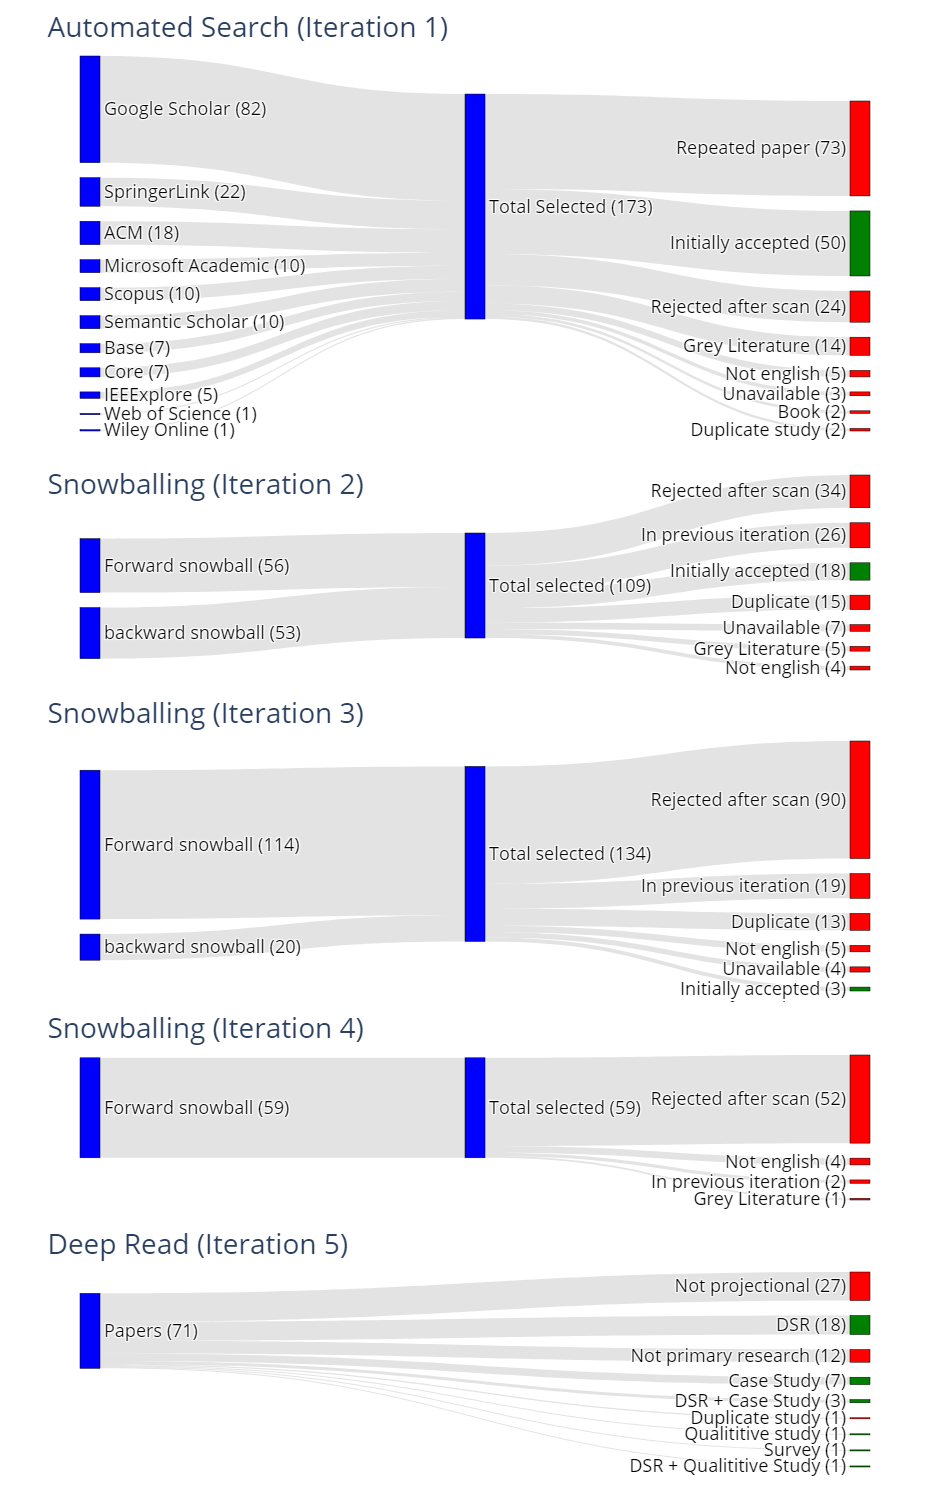
\includegraphics[width=0.95\textwidth]{Sections/images/search_sankey-2.png}}
    \caption{Search results}
    \label{fig:search_results}
\end{figure}

Our final selection iteration involved a deeper scan of the remaining 71 papers.
In this stage, we rejected 12 papers that were not primary research and one paper which reported on an already represented study.
Further, we rejected twenty-seven papers that were, on closer reading, not about projectional editing.

This final selection filter left us with 31 papers before the quality assessment filter. 

\subsubsection{Sensitivity and Precision}
As a curio, we reappropriated Zhang's\cite{Zhang_2011} ideas of sensitivity and precision and applied them to the search engines rather than search strings.
We calculate the values for sensitivity and precision of the search engines as follows:
\[
        sensitivity = \frac{\#\;retrieved\;relevant\;studies}{\#\;all\;relevant\;studies} \;100\%
\]

\[
        precision = \frac{\#\;retrieved\;relevant\;studies}{\#\;studies\;retrieved} \;100\%
\]

Table \ref{table:sensitivity_precision} show that Google Scholar had the highest sensitivity, returning 22 of the 31 chosen studies.
This sensitivity came at the cost of a considerable proportion of false positives.
Microsoft Academic and SpringerLink were the joint-most precise, with half of their search results ending up in the final roster.
With the second-highest count of documents, the second-highest sensitivity, and joint highest precision, SpringerLink would appear to be the best all-around search engine for this field.
However, these figures are skewed by several of their articles coming from a single collection specifically about projectional editing.

\begin{table}[h]
    \begin{center}
        \begin{tabular}{ | l | c | c | c | c |} 
            \hline
            Search engine/library     & original \# & selected \# & sensitivity & precision\\
            \hline
            \hline
            ACM                        & 18          & 3           & 10\%        &  16\%    \\
            BASE                       & 7           & 3           & 10\%        &  43\%    \\
            CORE                       & 7           & 1           &  3\%        &  14\%    \\
            Google Scholar             & 82          & 22          & 71\%        &  27\%    \\
            IEEExplores                & 5           & 2           &  6\%        &  40\%    \\
            Microsoft Academic         & 10          & 5           & 16\%        &  50\%    \\
            Science.gov                & 0           & 0           &  0\%        &   0\%    \\
            SCOPUS                     & 10          & 3           & 10\%        &  30\%    \\
            Semantic Scholar           & 10          & 4           & 13\%        &  40\%    \\
            SpringerLink               & 22          & 11          & 35\%        &  50\%    \\
            Wiley Online               & 1           & 0           &  0\%        &   0\%    \\
            Web of Science             & 1           & 0           &  0\%        &   0\%    \\
            \hline
        \end{tabular}
    \end{center}
    \caption{Search engine sensitivity and precision}
    \label{table:sensitivity_precision}
\end{table}

\subsection{Quality Assessment}
During this quality assessment, we discovered that two of the papers we had initially categorised as primary studies were, in fact, proposals, and thus we removed them from our analysis.
Using the quality assessment checklists developed by Crombie et al.\cite{crombie1997pocket}, shown in appendix \ref{appendix:QualityAssesmentChecklist}, we examined the remaining 29 papers, which on the surface represented 35 primary studies.

Unfortunately, there were no checklists for DSR studies.
We, unsuccessfully, searched for an appropriate quality assessment checklist for DSR studies.
We did not find a suitable checklist and did not consider ourselves suitably qualified to make one.
So, we used the quality assessment checklist for case studies to assess the DSR studies.

We used a rudimentary scoring system of +1 value for positive answers, 0 for undetermined, and -1 for negative answers.
We arbitrarily defined that any study with an overall score greater than 0 was high enough quality to be part of our final analysis.

Unfortunately, we only found 6 out of 37 studies of high enough quality to pass this filter with this scoring.
Thus, we had to choose between changing our scoring, only using these six studies, terminating the SLR or ignoring the QA findings.

Changing a method until it gave the desired answer seemed unscientific to us.
Six studies seemed too few to give an overview of a field.
Abandoning the SLA seemed the correct course of action.
However, as we still wanted an overview, we decided to take a different course.
We accept that what follows is no longer an SLA. 
We titled it a Quasi-SLA, which is like an SLA, which ignores the quality assessment results.

We could not reconcile that 84\% of studies were high-quality enough to appear in recognised scientific journals yet were not of high enough quality to pass our SLR QA stage.
After considering this disconnect, we found two significant threats to the validity of the Quality Assessment stage.
The first is that a single researcher with no previous experience executed the QA stage.
The second is that either case study checklists are inappropriate for DSR studies or that DSR studies are inappropriate for SLRs.

\subsection{Analysis}
\label{section:slr_analysis}

After Identifying the primary studies, we extracted data.
Appendix \ref{appendix:DataExtraction} shows the forms containing the raw extracted data.
Figure \ref{fig:study_types} shows that most of the primary studies in our review were DSR studies.

\begin{figure}[h]
    \centering
    \fbox{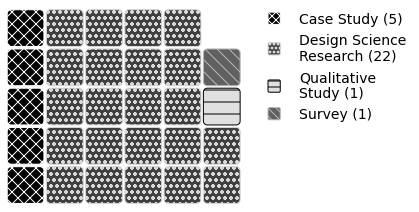
\includegraphics[width=0.45\textwidth]{Sections/images/pie_study_type4.png}}
    \caption{Study types}
    \label{fig:study_types}
\end{figure}

\subsubsection{Tools Used}

We split the studies to see which were to do with purely research projects and which were researching using already publicly available commercial or open-source products.
To calculate this, we removed one primary study, a survey, as it covered many tools and options, but none of which was in-depth.
Figure \ref{fig:public_vs_research} shows that over 80\% of the projects were studying already existing publicly available options.

Of the publicly available software studies, we wanted to know which software attracted the most academic interest.
Figure \ref{fig:public_programs} shows that 74\% of the studies into projectional editing that used a publicly available product used JetBrains MPS.

\begin{figure}[h]
    \centering
    \fbox{\begin{minipage}{0.5\textwidth}
            \centering
            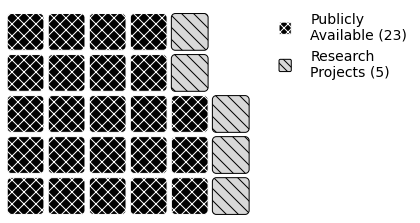
\includegraphics[width=0.85\textwidth]{Sections/images/pie_projectional_publicvsresearch3.png}
            \caption{Public vs research}
            \label{fig:public_vs_research}
        \end{minipage}\hfill
        \begin{minipage}{0.5\textwidth}
            \centering
            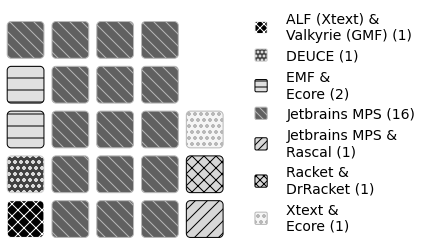
\includegraphics[width=0.85\textwidth]{Sections/images/pie_projectional_publicprograms3.png} 
            \caption{Publicly available programs}
            \label{fig:public_programs}
        \end{minipage}
    }
\end{figure}

\subsubsection{Sentiment}

In this study, we included all 29 papers.
We tagged each section from those papers that talked about projectional editing.
We then broke each section into sentences and ran those sentences through a sentiment analyser as described in section \ref{section:dataExtraction}.
We show the outcome of this sentiment analysis in figure \ref{fig:sentiment_analysis} on page \pageref{fig:sentiment_analysis}. 
The charts show the relationship between the positive, neutral, and negative sentiment outcomes.
On the y-axis, we have an Id for the papers examined. 
We show the keys linking the Ids to the paper names in table \ref{table:paper_key}, on page \pageref{table:paper_key}, the page following the charts.

\begin{figure}
    \centering
    \fbox{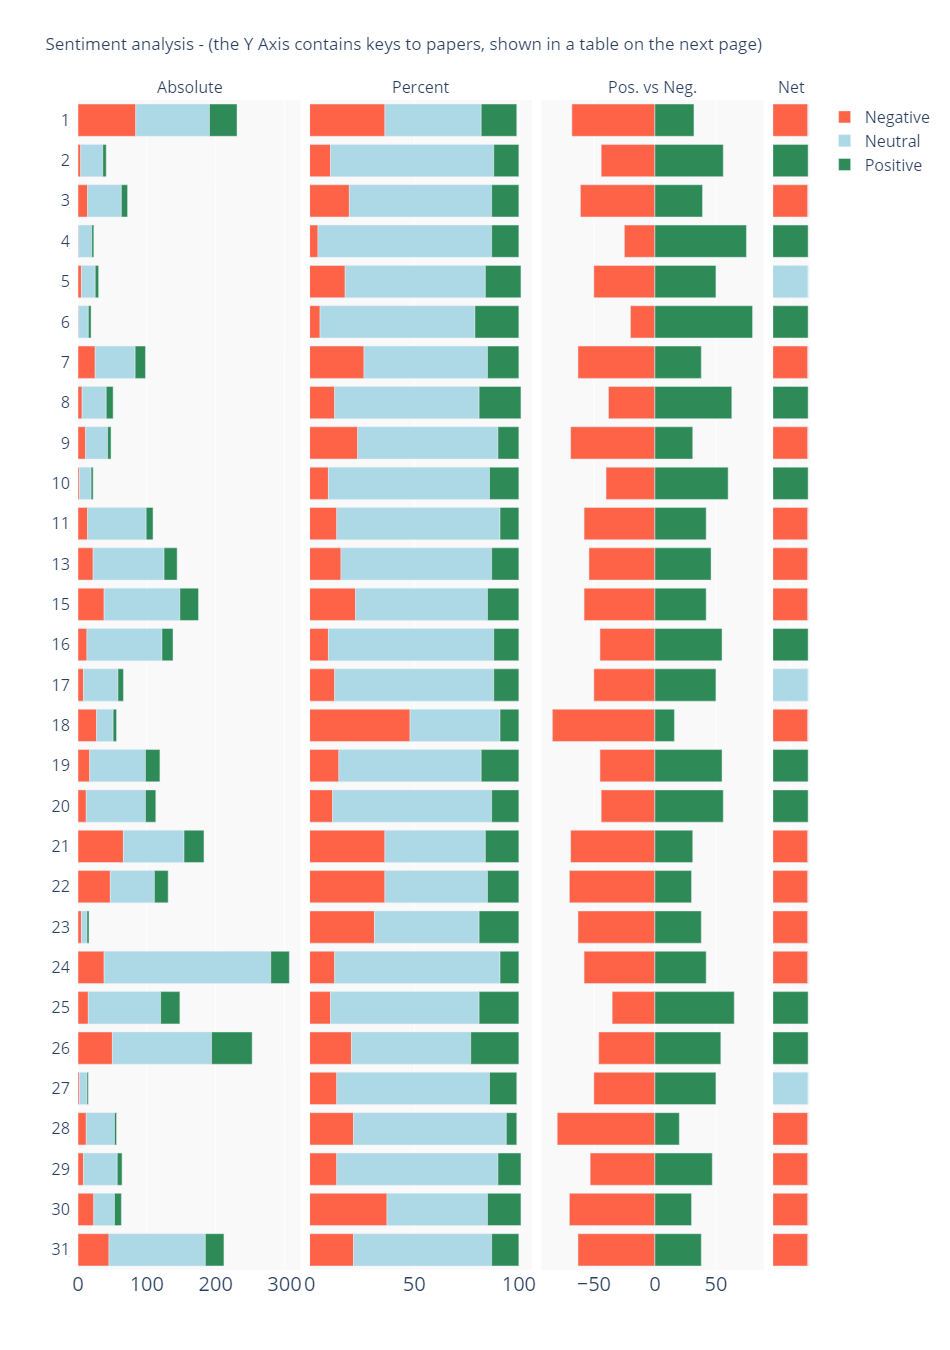
\includegraphics[width=0.95\textwidth]{Sections/images/sentiment_analysis4.png}}
    \caption{Sentiment analysis}
    \label{fig:sentiment_analysis} 
\end{figure}
 
\begin{table}
    \begin{center}
        \begin{tabular}{ |c  c|l | } 
            \hline
            Id  &                                        & Paper name                                                                  \\
            \hline
            1   &  \cite{voelterdomain_SLR}              & A domain-specific language for payroll calculations: A case study at DATEV  \\ \hline
            2   &  \cite{schropfer2021framework_SLR}     & A framework for projectional multi-variant model editors                    \\ \hline
            3   &  \cite{schropfer2020generic_SLR}       & A generic projectional editor for EMF models                                \\ \hline
            4   &  \cite{bucchiarone2019model_SLR}       & A model-driven approach towards automatic migration to microservices        \\ \hline
            5   &  \cite{meacham2020adaptivevle_SLR}     & AdaptiveVLE: An integrated framework for personalized online education      \\
                &                                        & using MPS JetBrains domain-specific modeling environment                    \\ \hline
            6   &  \cite{andersen2020adding_SLR}         & Adding interactive visual syntax to textual code                            \\ \hline
            7   &  \cite{addazi2021blended_SLR}          & Blended graphical and textual modelling for UML profiles: A                 \\
                &                                        & proof-of-concept implementation and experiment                              \\ \hline
            8   & \cite{meacham2020classification_SLR}   & Classification algorithms framework (CAF) to enable intelligent systems     \\
                &                                        & using JetBrains MPS domain-specific languages environment                   \\ \hline
            9   & \cite{furtado2021dsl_SLR}              & DSL based approach for building model-driven questionnaires                 \\ \hline
            10  & \cite{beckmann2020efficient_SLR}       & Efficient editing in a tree-oriented projectional editor                    \\ \hline
            11  & \cite{kolovos2020efficient_SLR}        & Efficient generation of graphical modelviews via lazy model-to-text         \\
                &                                        & transformation                                                              \\ \hline
            13  & \cite{bucchiarone2021engineering_SLR}  & Engineering gameful applications with MPS                                   \\ \hline
            15  & \cite{ratiu2021fasten_SLR}             & Fasten: An extensible platform to experiment with rigorous modeling of      \\
                &                                        & safety-critical systems                                                     \\ \hline
            16  & \cite{lafontant2020gentleman_SLR}      & Gentleman: A light-weight web-based projectional editor generator           \\ \hline
            17  & \cite{schropfer2019integrating_SLR}    & Integrating UML and ALF: An approach to overcome the code generation        \\
                &                                        & dilemma in model-driven software engineering                                \\ \hline
            18  & \cite{santos2020javardise_SLR}         & Javardise: A structured code editor for programming pedagogy in Java        \\ \hline
            19  & \cite{schindler2021jetbrains_SLR}      & JetBrains MPS as core DSL technology for developing professional digital    \\
                &                                        & printers                                                                    \\ \hline
            20  & \cite{simi2021learning_SLR}            & Learning data analysis with metaR                                           \\ \hline
            21  & \cite{stotz2021migrating_SLR}          & Migrating insurance calculation rule descriptions from Word to MPS          \\ \hline
            22  & \cite{munk2020model_SLR}               & Model-based safety assessment with SYSML and component fault trees:         \\
                &                                        & Application and lessons learned                                             \\ \hline
            23  & \cite{bucchiarone2020papyrus_SLR}      & Papyrus for gamers, let’s play modeling                                     \\ \hline
            24  & \cite{merino2021projecting_SLR}        & Projecting textual languages                                                \\ \hline
            25  & \cite{cuinat2020specedit_SLR}          & SpecEdit: Projectional editing for TLA+ specifications                      \\ \hline
            26  & \cite{prinz2021teaching_SLR}           & Teaching language engineering using MPS                                     \\ \hline
            27  & \cite{barash2021teaching_SLR}          & Teaching MPS: Experiences from industry and academia                        \\ \hline
            28  & \cite{hempel2020tiny_SLR}              & Tiny structure editors for low, low prices! (generating GUIs from           \\
                &                                        & toString functions)                                                         \\ \hline
            29  & \cite{negm2020towards_SLR}             & Towards ontology-based domain specific language for internet of things      \\ \hline
            30  & \cite{lubin2020type_SLR}               & Type-directed program transformations for the working functional            \\
                &                                        & programmer                                                                  \\ \hline
            31  & \cite{ozkaya2021practitioners_SLR}     & What do practitioners expect from the meta-modeling tools? a survey         \\ \hline
        \end{tabular}
    \end{center}
    \caption{Paper key}
    \label{table:paper_key}
\end{table}

The charts in the first column of figure \ref{fig:sentiment_analysis} show the absolute number of sentences analysed per paper partitioned by whether they returned negative, neutral, or positive sentiment results.
The charts in the second column show these as percentages so that the papers are comparable.
In the charts in the third column, we removed the neutral scores and calculated the percentage positive to negative.
The final chart column is an aid to make it easier to scan whether papers trended positive or negative.
If we found the papers to be equally positive and negative, we classified them as neutral.

Over the 29 papers, we scanned a total of 3003 sentences.
Four hundred thirty-five were analysed as being positive, 1953 were neutral, and 615 were negative.
Hence, 14\% were positive, and 16\% were negative.

10 of the 29 papers were more positive than negative when discussing projectional editing, 16 more negative and three equally negative and positive.

In figure \ref{fig:sentiment_analysis2}, we attempt to separate sentiment by product category.  
These categories are Research projects, MPS, and all the other used products.
We ignored the survey paper in this one as it covered all these types.

\begin{figure}[H]
    \centering
    \fbox{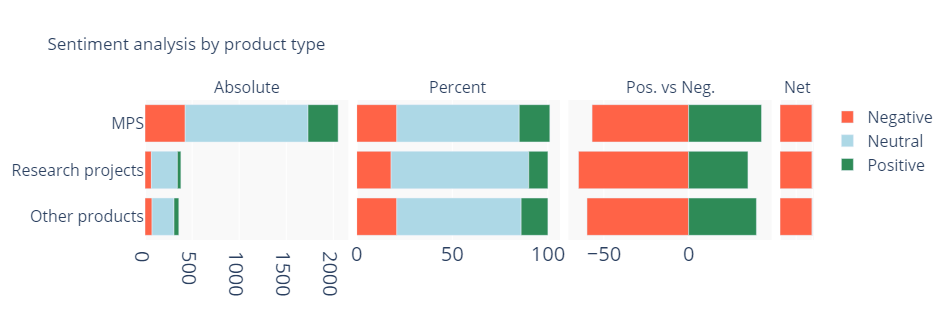
\includegraphics[width=0.95\textwidth]{Sections/images/sentiment_analysis2_2.png}}
    \caption{Sentiment analysis by product}
    \label{fig:sentiment_analysis2}
\end{figure}

MPS dominates the sentences accounting for 17 (61\%) of the 28 papers and 2051 (73\%) of the 2791 sentences analysed.

\subsubsection{A Narrative Synthesis}
Our synthesis of the papers that appear in table \ref{table:paper_key} will be short.
We will avoid rehashing the advantages and disadvantages of projectional editing, which come up again as we discussed these thoroughly in sections \ref{section:projectional_advantages} and \ref{section:projectional_disadvantages}.

Many of these papers focus on models and model-driven development, occasionally suggesting a shift towards textual modelling languages.
However, other papers point out that text does not always supply a suitable level of abstraction in modelling.
One paper suggested that developers prefer text, whereas maintainers and domain experts prefer visual projections, though this suggestion was unsourced.

When authors have used solutions other than MPS, they complain about issues such as MPS being heavyweight, with much overhead.
However, these authors then spend a great deal of time theorising about fixing issues in their architecture which, because of its architecture, MPS does not encounter.
These issues include synchronising between various views and how grammars deal with notations.

There is a fair bit of mention of a ``semi-projectional'' approach, which involves parsing at the leaf node level of the AST.
This approach is mainly from papers not using MPS, but also some which do.
The approach, it seems, is a reaction to the difficulty in simulating the text language experience in a projectional editor. 
It echoes the approach the Synthesizer Generator adopted when facing this same problem in the 80s.

The projects they describe are not in industrial use.
These authors suggest that projectional editing is probably best suited to helping novices learn a language. 

Those authors who use MPS primarily discuss products developed for use in an industrial setting or how best to teach projectional editing to a broader audience.
MPS, when used, is often seen as a critical enabler.
Two of MPS' properties that garner the most mentions are the ease of composition and multiple views.

The users of MPS agree that simulating the experience of the text editor user in the projectional environment is still very hard.
However, new plug-ins are making this somewhat more manageable.
The most prominent carrion call amongst the MPS users is for a web-based interface.

The steep learning curve is another issue.
Several papers offer solutions to this, such as example-driven development, gamification, grammar to MPS plug-ins and something called a ``language wheel''.

In general, researchers using MPS have a few gripes with usability but seem to be very positive.
One paper, which was not using MPS, said that some problems become intractable when dealing with graphical models.
Another paper, in a coincidence of word use, when describing the decision to use MPS, explained that it was because it presented a tractable level of complexity. 


\section{Discussion}
\label{section:slr_discussion}

We now examine threats to the construct, the internal and external validity of our SLR, its reliability, and areas of improvement.

 
\subsection{Threats To Validity}  
As discussed in their tertiary study of SLRs, da Silva et al.\cite{DaSilvaFabioQ.B2011Syos}, one of the main problems of SLRs in Software engineering is a focus on practice and not experimentation.
Because of the nature of the subject area, we will be making this same shortfall. 
We feel that we have fully addressed their other concerns of SLRs not assessing the quality of our primary studies, bad integration and lack of guidelines.

As with all SLRs, the main threats to validity are an incomplete set of studies due to an insufficient search strategy, researcher bias in paper selection and inaccuracy in data extraction.
In our study quality assessment, we used Runeson et al.'s\cite{runeson2009guidelines} four suggested limitations of studies, namely construct validity, internal validity, external validity, and reliability.
It is only fair that we point this towards our study.

\subsubsection{Construct Validity}
Regarding construct validity, i.e., whether our research questions match the research subjects methods and measures, whilst no measurement system is perfect, some are much further from perfect than others.

For the construct to be valid, we need to present the best available evidence.
The nature and modernity of projectional editing might mean plenty of good evidence is available in grey literature and industrial articles. 
This under-representation of actual but non-academic studies could lead to a false positive or negative for some of the questions, leading to errors in recommendations.

There may be circumstances that influence the best evidence, such as who is funding the study. 
Is a researcher working or consulting at a projectional editing product supplier, and will this skew results.

Are some projectional editors being ignored because of the preference for English papers only?
The focus on English language papers might be biased against projectional editors aimed at non-English speaking markets.

The use of the sentiment analysis tool may have been inappropriate.
Scientific papers may not lend themselves to sentiment analysis in general.
The Azure sentiment analysis service may not be appropriate for scientific papers.

\subsubsection{Internal Validity}
Internal validity, or the causal relationships, questions whether one factor causes an effect or are both factors influenced by something unseen.

An incomplete search term may have lead to selection bias.  
Using ``projectional editing'' and ``projectional editor'' may have led us into a small corner of this field.
If one tool uses this term and others use other terms to describe a similar approach, these search terms may misrepresent the field.
Other tools or projects could use different terms, such as ``language orientated programming'' or more antiquated terms like ``structured programming'' or ``syntax-directed editing''.

One causal relationship that could have influenced the outcome was that the book ``Domain-Specific Languages in Practice with JetBrains MPS'' was published right at the end of our selection period.
Of the 11 papers published in this book, 7 made it into our final paper selection.
As this book is all studies involving using MPS, then this skews the data towards MPS.

We also had an error with the identification of primary studies. 
Initially, we took the word of the paper when it said it had done a case study, but frequently, that just meant trying their code out on a current problem rather than a case study in the academic sense.

A final threat to internal validity was that no expert in either Drools or projectional editing evaluated the conclusions we drew.

\subsubsection{External Validity}
External validity is the ability to generalise the findings.

The prevalence of the DSR methodology in software engineering is why these results are impossible to generalise.
The ``primary study'' data in these cases are often just the source code.

Another threat to validity is whether this is a good representation of the field is our restricted timespan of the search, would the findings be similar across a longer time frame.
However, as the scope of the question was to examine the current state, we still feel that this restriction is necessary and informative.

\subsubsection{Reliability}
Reliability is how the data and the analysis is dependant on specific researchers.
Here we are presented with a very credible threat in that a single researcher carried out this research.
Under particular threat from the single-researcher bias were the quality assessments. 

Whilst measures were put in place to try and mitigate this, the reliance on a single person's judgement of the underlying studies leaves the door to bias wide open.
Another threat is the use of narrative review. 
This review type can be subjective and, therefore, difficult to reproduce.

As mentioned in the results, we were not happy with any of the paper quality assessments for DSR studies.
Using an inappropriate quality assessment tool was instrumental in the almost complete failure of the quality assessments.


\subsubsection{Repeatability Vs Reproducibility}
Greenhalgh et al.\cite{GreenhalghTrisha2005Eaeo} in their review of where papers come from in SLRs, found that 24\% of papers come from "personal knowledge or personal contact".
For the sake of reproducibility, we decided not to hunt down relevant papers from knowledgeable people in the field, as this would require anyone trying to reproduce this study to ask the same people at the same knowledge level as us.

\subsubsection{Method Improvement}
An area we would improve is sentiment analysis.
Our technique was flawed.
To avoid the risk of bias through us cherry picking paragraphs, we were very coarse-grained in our input selection criteria.
For all papers, we chose the introduction, the conclusion and then any section that discussed anything to do with projectional editing.

The problem is that sometimes the sections would run for paragraphs, with only one or two being about projectional editing.
Frequently, especially with papers involving MPS, the paper was focused on a problem and using MPS to solve it.
Thus, the introductions and conclusions would occasionally barely mention projectional editing.

If we were to do this again, we would take a more fine-grained approach as we feel the cherry-picking risk is less significant than the noise from the unrelated text.



\section{Summary}
In this chapter, we presented a description of the details of the SLR we conducted.
The quality assessment filter was not adequate for the task of this review. 
Thus, the review did not follow the methodology design completely.
Looking only at papers created in the 18 months prior to conducting the review, 29 papers met our criteria.

A large majority of these papers were design science research studies.
JetBrains MPS was the tool used for most of the papers.
Papers using MPS focused on industrial and educational use, whereas those not using MPS mainly experimented with the projectional form.

We ran sentiment analysis on these papers. 
Results were inconclusive.

Two areas of improvement would be to design a better quality assessment filter and to improve the data cleaning for the sentiment analysis.